\documentclass{beamer}
\setbeamertemplate{navigation symbols}{}
\setbeamertemplate{caption}{\insertcaption}

\usetheme{Dresden}
\usecolortheme{crane}

\usepackage{amsmath}
\graphicspath{{figs/}}
\usepackage{multirow}

\usepackage{tikz}

\let\Tiny\tiny
\usepackage{graphicx}
\usepackage{xmpmulti}
\usepackage{multimedia}
%\usepackage{media9}


\beamersetuncovermixins{\opaqueness<1>{25}}{\opaqueness<2->{15}}

\begin{document}
	\title{Natural language Processing}  
	\author{Saumya Bhatnagar}
	\date{\today} 
	
	
\begin{frame}
\titlepage
\end{frame}

\begin{frame}[allowframebreaks]\frametitle{Table of contents}\tableofcontents
\end{frame} 





\section{Components of NLP}

\begin{frame}\frametitle{General}
	\textbf{Text Mining}: process of deriving high quality information from texts\\
	Turn text into data for analysis via NLP\\
	NLP (AI): deals with human languages\\
	what is inflection?\\
	
	
\end{frame}




\begin{frame}%[plain]
	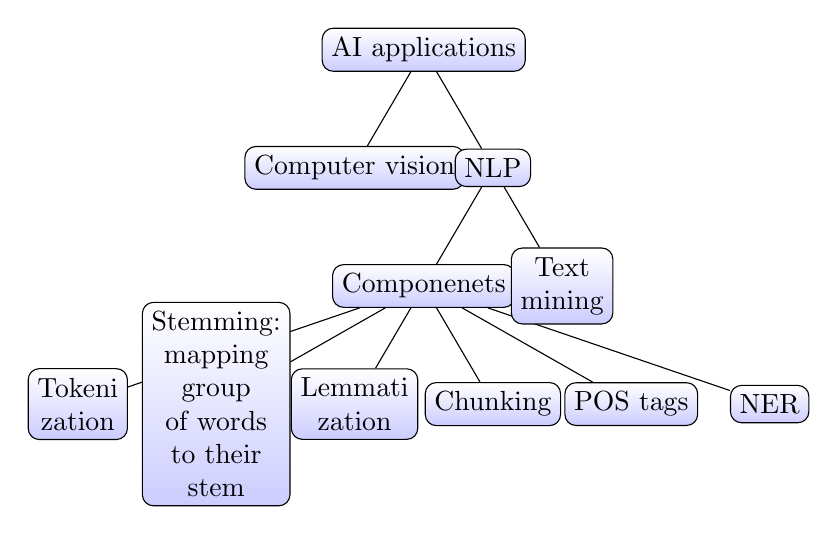
\begin{tikzpicture}[
	sibling distance=5em,
	every node/.style = {
		shape=rectangle, rounded corners,
		draw, align=center,
		top color=white, bottom color=blue!20}]]
	\node {AI applications}
	child { node {Computer vision} }
	child { node {NLP}
		child { node {Componenets}
			child { node {Tokeni\\zation} }
			child { node {Stemming:\\mapping\\group\\of words\\to their\\stem} }
			child { node {Lemmati\\zation} } 
			child { node {Chunking} } 
			child { node {POS tags} } 
			child { node {NER} } 
		}
		child { node {Text\\mining} } 
	};
	\end{tikzpicture}
\end{frame}

\begin{frame}\frametitle{Tokenizer}
	break sentences into words\\
	
\end{frame}

\begin{frame}\frametitle{Stemming and Lemmatization}
	\begin{columns}
		\begin{column}{0.5\textwidth}
			\textbf{Stemming}\\
			Might not be an actual word\\
			Predefine steps\\
			Speed is imp\\
		\end{column}
		\begin{column}{0.5\textwidth}
			\textbf{Lemmatization}\\
			Returns an actual word\\
			Uses WordNet corpus\\
			Language is imp\\
		\end{column}	
	\end{columns}

	\textbf{Stemming}: Stem word might not be an actual word\\
	\begin{itemize}
		\item 	Porter stemmer: based on 5 pre-defined rules, simple and fast, mainly used in IR (information retreival) search queries
		\item Snow-ball stemmers: by NLTK, has non-english stemmers (french, german, english, italian,)
		\item 	Lancaster stemmer: Iterative, over-stemming may occur, shorter stem then Porter
		\item ISRI Stemmer
		\item RSLPS Stemmer
	\end{itemize}

\end{frame}

\section{Topic Modeling/Document clustering}
\begin{frame}\frametitle{bayesian Modeling}
	content...
\end{frame}

\section{Sentiment Analysis}
\begin{frame}\frametitle{}
content...
\end{frame}

\section{Information Retrieval}
\begin{frame}\frametitle{}
content...
\end{frame}

\begin{frame}
	Thank You!
\end{frame}

\end{document}